\documentclass{article}
\usepackage[utf8]{inputenc}
\title{Actividad 6}
\author{Roberto Alexis Gómez Pintor}
\usepackage{graphicx}
\usepackage{float}
\begin{document}
\maketitle
\section{Introduccion}
En esta actividad se aborda el modelo de dos resortes acoplados con el fin de
utilizar las funciones de jupyter lab para resolver las ecuaciones correspondientes
y poder encontrar el comportamiento gráfico de estos resortes bajo diferentes
circunstancias.
\section{Sistemas de 2 resortes acoplados}
El modelo consiste entre 2 resortes y 2 masas, el resorte 1 esta sujeto a una pared y tiene una masa (m1), el resorte 2 esta conectado a la masa 1 y la masa 2 (m2) esta conectado al resrote 2. En el artículo que se ha revisado se investiga el problema que aparece alejado de la corrección práctica para ser incluido únicamente como una descripción en los libros de texto. Esto es el problema de recurrir con dos masas unidas en serie que cuelgan de un techo, en el cual se asume que las fuerzas se comportan de acuerdo con la Ley de Hooke. Este problema se resuelve con ecuaciones diferenciales lineales de segundo orden. Se puede investigar cuando el movimiento de las masas está sincronizado o en fase y cuando se oponen entre sí a 180 grados fuera de fase, esto se a logrado modificando las constantes del resorte.
\begin{figure}[!ht]
\centering
\includegraphics[width=0.3\textwidth]{two_springs.png}
  \caption{Ley de Hooke.}
\end{figure}
\section{Modelo de resortes acoplados}
El modelo se constituye en 2 resortes y 2 masas, con 2 constantes llamadas k1 y k2, estas se colocan respectivamente este se coloca del techo y el peso de la masa
m1 se une teniendo un resorte en su parte inferior al cual se le agrega la masa
m2. Permitiendo que el sistema llegue a un punto de equilibrio, se mide el
desplazamiento del centro de masa de cada una de las masas a partir del equilibrio
1como una función del tiempo y se denotan estas medidas como X1 (t) y x2 (t)
respectivamente. Se asume que las fuerzas restitutivas son de la forma -k1l1 y -k2l2 donde l1 y l2 son las compresiones de los dos resortes.

Debido a que la masa superior esta unida a dos resortes, existen dos fuerzas restitutivas actuando sobre ella dadas como consecuencias de -k1x1 y -k2(x2-x1), mientras que la segunda masa solo siente la fuerza correspondiente debido al segundo resorte.
\section{Apendice}
\subsection{¿En general te pareció interesante esta actividad de modelación matemática? ¿Qué te gustó mas? ¿Qué no te gustó?}
El desarrollo de la ley de Hooke y lo que no me agrado fue uno que otro problema en el codigo que me genero un tiempo perdido.
\subsection{La cantidad de material te pareció ¿bien?, ¿suficiente?, ¿demasiado?}
 Fue bastante.
\subsection{¿Cuál es tu primera impresión de Jupyter Lab? R:Bastante util la herramienta.}
\subsection{Respecto al uso de funciones de SciPy, ¿ya habías visto integración numérica en tus cursos anteriores? ¿Cuál es tu experiencia?.}
No fueron usadas ni vistas, al experiencia es nula.
\subsection{El tema de sistema de masas acopladas con resortes, ¿ya lo habías resuelto en tu curso de Mecánica 2?}
Fue estudiado y habia resueltos unos cuantos problemas similares.
\subsection{¿Qué le quitarías o agregarías a esta actividad para hacerla más interesante y divertida?}
EL uso de varias ecuaciones para disminuir la carga de contenido, pero aparte de eso no encuentro otra cosa que modificar.
\section{Graficas}
\begin{figure}[!ht]
\centering
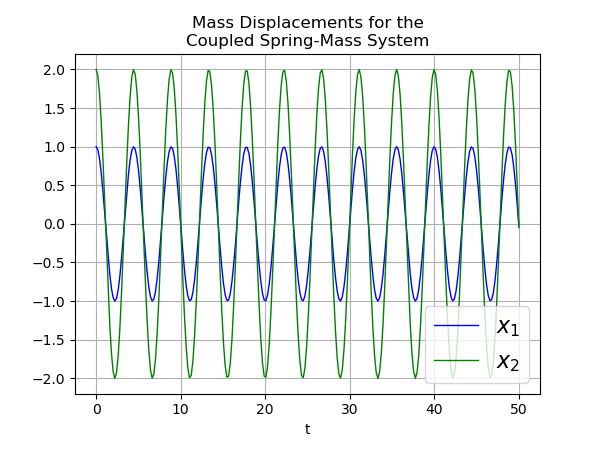
\includegraphics[width=0.8\textwidth]{two_springs1-1.png}
\end{figure}
\begin{figure}[!ht]
\centering
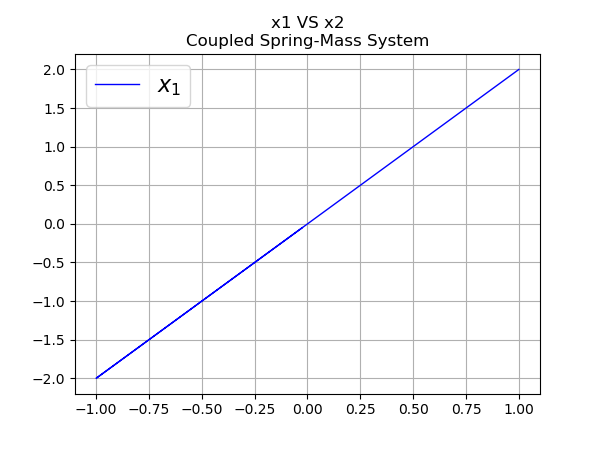
\includegraphics[width=0.8\textwidth]{two_springs1-2.png}
\end{figure}
\begin{figure}[!ht]
\centering
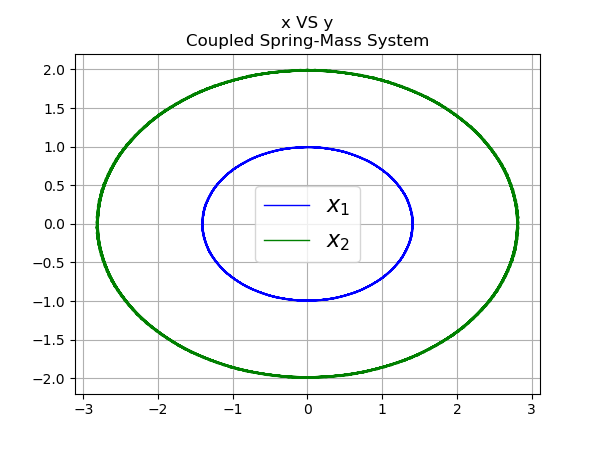
\includegraphics[width=0.8\textwidth]{two_springs1-3.png}
\end{figure}
\begin{figure}[!ht]
\centering
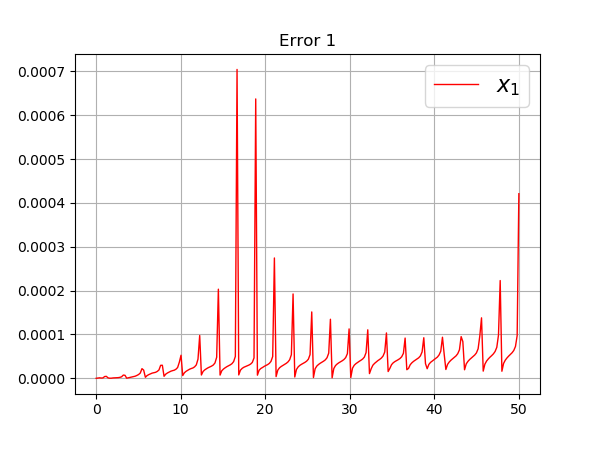
\includegraphics[width=0.8\textwidth]{two_springs1-E1.png}
\end{figure}
\begin{figure}[!ht]
\centering
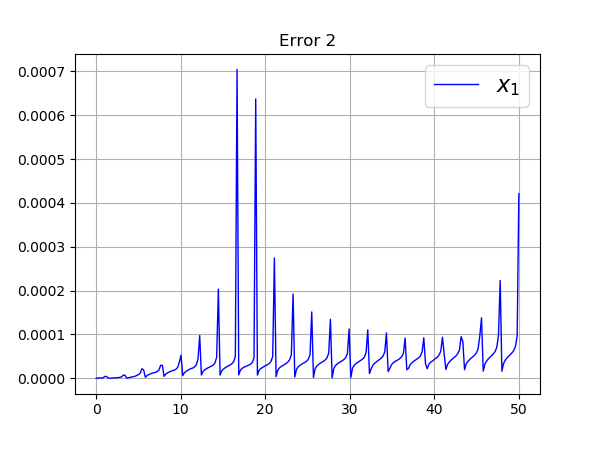
\includegraphics[width=0.8\textwidth]{two_springs1-E2.png}
\end{figure}
\begin{figure}[!ht]
\centering
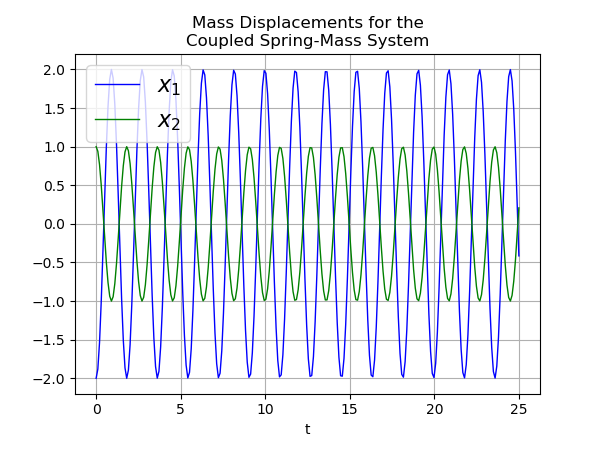
\includegraphics[width=0.8\textwidth]{two_springs2-1.png}
\end{figure}
\begin{figure}[!ht]
\centering
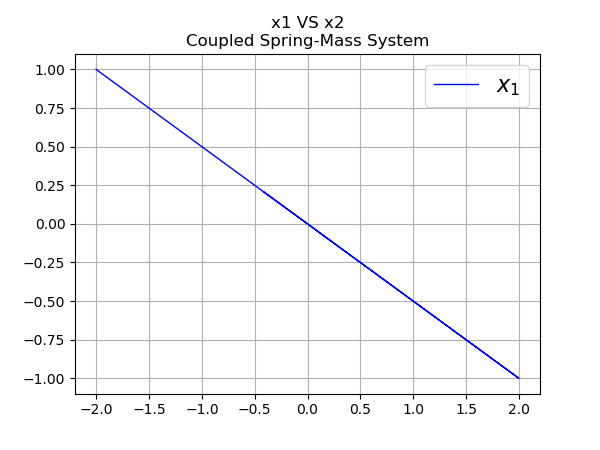
\includegraphics[width=0.8\textwidth]{two_springs2-2.png}
\end{figure}
\begin{figure}[!ht]
\centering
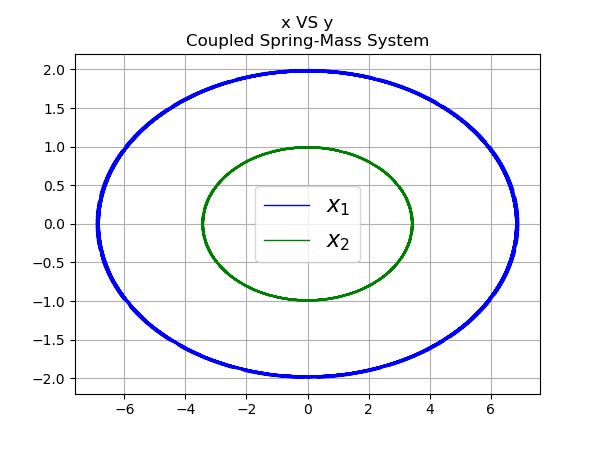
\includegraphics[width=0.8\textwidth]{two_springs2-3.png}
\end{figure}
\begin{figure}[!ht]
\centering
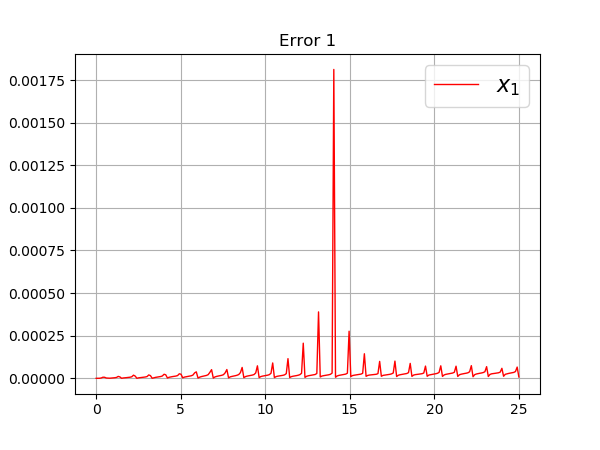
\includegraphics[width=0.8\textwidth]{two_springs2-E1}
\end{figure}
\begin{figure}[!ht]
\centering
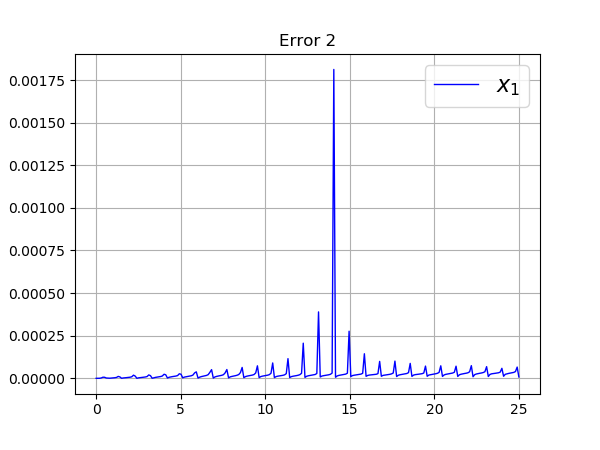
\includegraphics[width=0.8\textwidth]{two_springs2-E2}
\end{figure}
\begin{figure}[!ht]
\centering
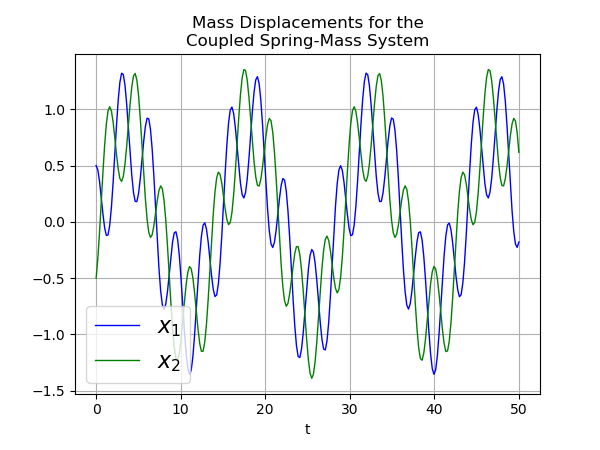
\includegraphics[width=0.8\textwidth]{two_springs3-1}
\end{figure}
\begin{figure}[!ht]
\centering
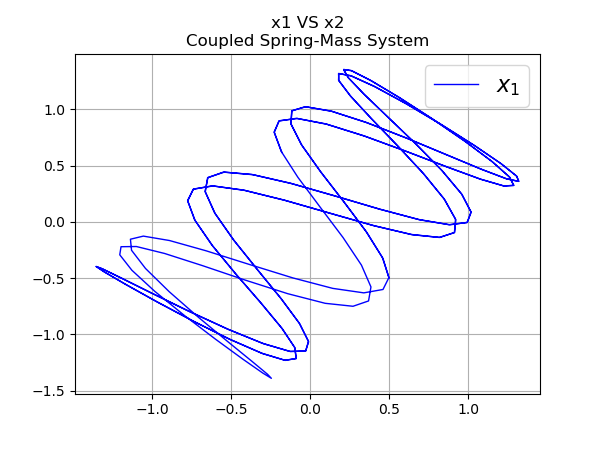
\includegraphics[width=0.8\textwidth]{two_springs3-2}
\end{figure}
\begin{figure}[!ht]
\centering
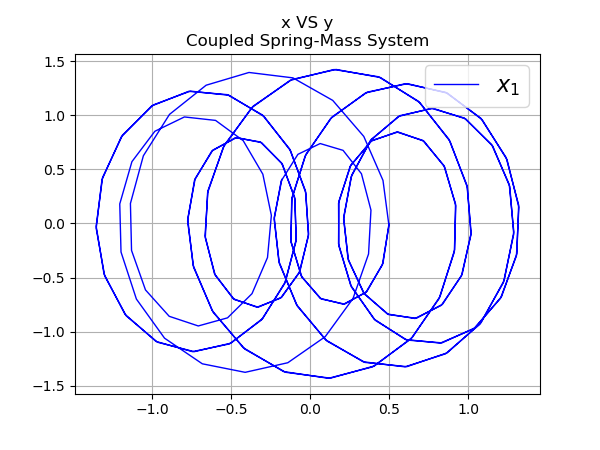
\includegraphics[width=0.8\textwidth]{two_springs3-3}
\end{figure}
\begin{figure}[!ht]
\centering
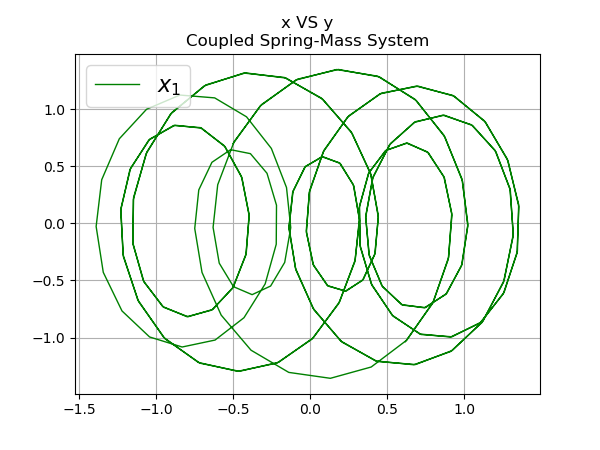
\includegraphics[width=0.8\textwidth]{two_springs3-4}
\end{figure}
\begin{figure}[!ht]
\centering
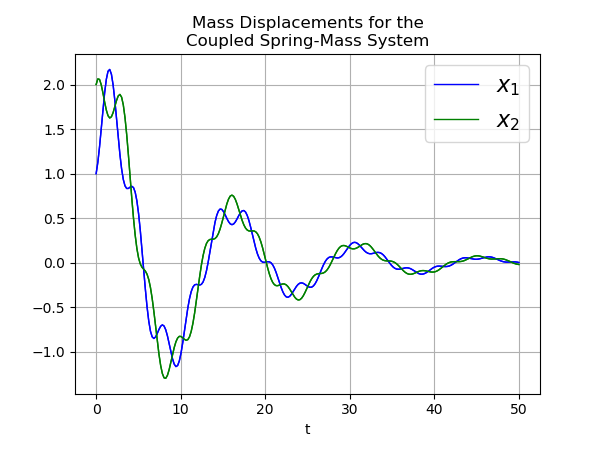
\includegraphics[width=0.8\textwidth]{two_springs4-1}
\end{figure}
\begin{figure}[!ht]
\centering
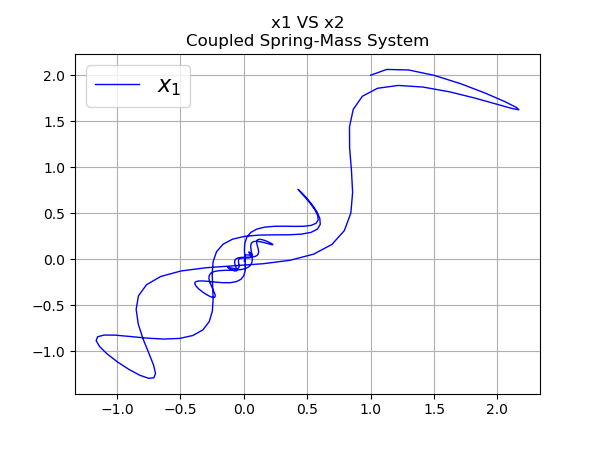
\includegraphics[width=0.8\textwidth]{two_springs4-2}
\end{figure}
\begin{figure}[!ht]
\centering
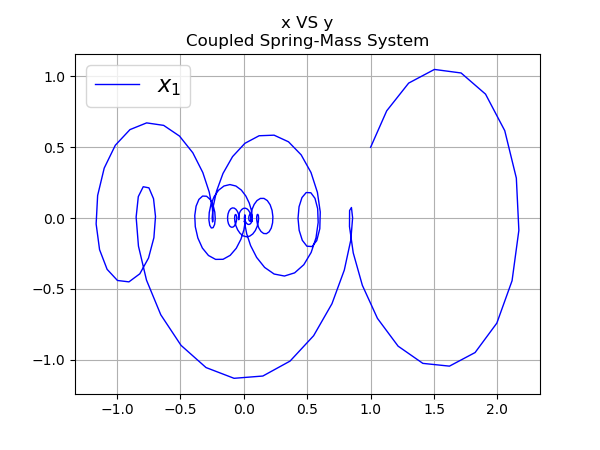
\includegraphics[width=0.8\textwidth]{two_springs4-3}
\end{figure}
\begin{figure}[!ht]
\centering
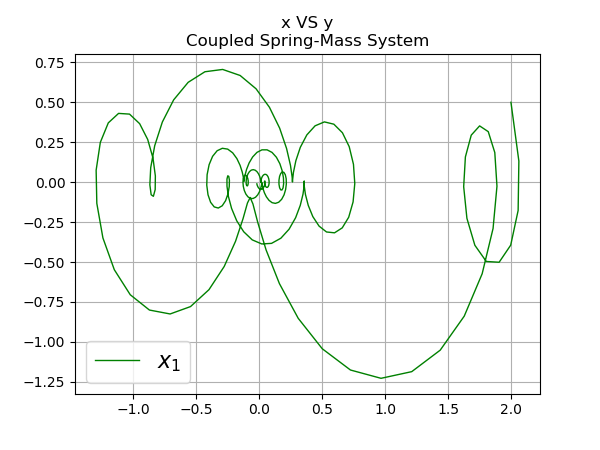
\includegraphics[width=0.8\textwidth]{two_springs4-4}
\end{figure}

\end{document}